\documentclass{exam}

\usepackage{graphicx}
\usepackage{amssymb}
\usepackage[T1]{fontenc}
% \usepackage{wrapfig}

\graphicspath{ {../res/} }

\title{Triathlon - Maths}
\author{Olympiad Maths}
\date{April 2022}

\pagestyle{plain}
\marksnotpoints

\begin{document}
\large
\maketitle

\begin{center}
    \vspace{-10pt}
    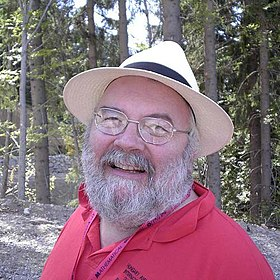
\includegraphics[height=100pt]{geoffsmith}
    \vspace{-10pt}
\end{center}

\section* {Instructions}

Read these before attempting the questions.

\subsection*{Time: 4.5 hours}

\subsection*{Format}
This paper has 7 available questions worth different numbers of marks. Only your best 3 questions (highest number of marks) will be counted.\\
Full written proofs are needed to gain marks.

\subsection*{Knowledge required}
Standard olympiad/BMO knowledge - problem-solving skills are most important.\\
\textbf{No calculators.}

\subsection*{Submission}
Submit your paper by dm to
{\fontfamily{cmss}\selectfont e=pi=3\#5257}
before \textbf{23:59 on XXXX}.\\
Please scan in then send as a \textbf{single PDF}. Online tools are available for this.\\
On the front page, write your \textbf{discord ID} (right click username -> copy ID).\\
After submission, you can be added to a channel to discuss the questions. Please don't discuss them outside of that channel.

\centering

\vspace{\stretch{1}}
\textbf{The questions begin on the next page.}\\
\vspace{10pt}
Good luck, and most importantly have fun!
\vspace{\stretch{1}}



\newpage
\section*{Questions}
\vspace{20pt}

\begin{questions}
    \question[20]
    Alice and Bob play a game of "21 dares". They collectively count from 1 to 21 in sequence, alternating the person who speaks. When speaking, they can either say 1, 2, or 3 consecutive numbers. The person who says 21 loses, and Alice goes first.
    \begin{parts}
    \part
    Show that Bob can always win.
    \part
    Alice now thinks this is unfair, and wants to play "420 dares" instead (same rules, but replace all instances of 21 with 420). Does anyone have a winning strategy?
    \part
    Who wins in a game of "$n$ dares"?
    \end{parts}
    \vspace{\stretch{1}}

    \question[40]
    Find all solutions in positive integers to the equation:
    \[ y^2(x-1) = x^5 - 1 \]

    \question[40]
    In triangle $ABC$, $M$ is the midpoint of $BC$. Let $P$ be a point on $AM$, inside triangle $ABC$.
    Rays $BP$ and $CP$ meet segments $AC$ and $AB$ at $D$ and $E$ respectively. Let the circles with diameters $BD$ and $CD$ meet at $X$ and $Y$.

    Show that $A, X, Y$ are collinear.
    \vspace{\stretch{1}}

    \question[50]
    Find all functions $f : \mathbb{Z} \mapsto \mathbb{Z}$ such that for all $a, b \in \mathbb{Z}$:
    \[ f(2a) + 2f(b) = f(f(a+b)) \]

    \question[50]
    Let $ABC$ be an acute-angled triangle with circumcircle $\gamma$. The tangents to $\gamma$ at $B$ and $C$ meet at $P$, and $AP$ intersects $\gamma$ again at $Q$.
    Let the angle bisector of $B \hat A C$ meet $BC$ at $D$ and $\gamma$ again at $E$.

    Show that $D \hat Q E$ = 90.
    \vspace{\stretch{1}}

    \question[60]
    Define the sequences $x_n, y_n$ as follows:
    \begin{itemize}
        \item
        $x_0 = 1, y_0 = 2$
        \item
        $x_{n+1} = \frac{x_n + y_n}{2}$
        \item
        $y_{n+1} = \sqrt{x_{n+1}y_n}$
    \end{itemize}

    Find $\lim_{n \to \infty} y_n$.

    \question[60]
    There is a regular $n$-gon with all diagonals drawn ($n \geq 3$). Assign the number 1 to every vertex and internal intersection of diagonals.
    A "move" consists of flipping the signs of all numbers along a particular side or diagonal.

    For which $n$ is it possible to perform a series of moves that changes all the 1s to -1s?
    \vspace{\stretch{1}}

\end{questions}


\vspace{\stretch{1}}
\centering \LARGE \textbf{END OF PAPER}
\vspace{\stretch{1}}
\end{document}